\documentclass[11pt]{article}
\synctex=1
 \expandafter\let\csname equation*\endcsname\relax
 \expandafter\let\csname endequation*\endcsname\relax
\usepackage{bm}
\usepackage{enumerate}
\usepackage[top=1in, bottom=1in, left=1in, right=1in]{geometry}
\usepackage{mathrsfs,color}
\usepackage{amsfonts}\usepackage{multirow}
\usepackage{amssymb}
\usepackage{amsmath}
\usepackage{float}
\usepackage{graphicx,afterpage}
\usepackage{epstopdf}
\usepackage[pdftex,colorlinks=true]{hyperref}
\usepackage[sort,compress]{cite}

\usepackage{natbib}
\usepackage{upgreek}
\usepackage{xcolor} 
\usepackage{bm}
\usepackage{algorithm2e} 

\usepackage{tikz}
\def\checkmark{\tikz\fill[scale=0.4](0,.35) -- (.25,0) -- (1,.7) -- (.25,.15) -- cycle;}

\usepackage{xcolor}
\usepackage{tikz}

\hypersetup{
     colorlinks   = true,
     citecolor     = black,
     linkcolor     = black
}


\newcommand{\EqRef}[1]{(\ref{#1})}




\begin{document}
\title{Matlab tutorials for Math 313 at the University of Arizona}
\author{M.~Morzfeld}
\maketitle

\section{Introduction}
The tutorials illustrate how to use Matlab to
implement some of the techniques you learn about in class.
In total, there are seven Tutorials:
\begin{itemize}
	\item
	Tutorial 0 -- Matlab basics
	\item
	Tutorial 1 -- Row-reduction 
	(Chapter~1)
	\item
	Tutorial 2 -- Matrix algebra, LU factorization, inverse, Leontief model
	 (Chapter~2) 
	\item
	Tutorial 3 -- Markov chains
	(Chapter~4.9)
	\item
	Tutorial 4 -- Eigenvalues, eigenvectors and diagonalization
	(Chapter~5)
	\item
	Tutorial 5 -- The power method for computing eigenvalues
	(Chapter~5.8)
	\item
	Tutorial 6 -- Least-Squares
	(Chapter~6)
	\item
	Tutorial 7 -- Singular value decomposition
	(Chapter~7.4)
\end{itemize}
\noindent
Here, the chapter refer to chapter in the text book:
\begin{center}
	D.C.~Lay, S.R. Lay, J.J.~McDonald\\
	Linear Algebra and its Applications	\\
	5th Edition, Pearson, 2016 
\end{center}

\noindent
The tutorials are ``\emph{live scripts}'', 
which means that they are a combination of text, equations and code.
When working on a tutorial, you should read the text carefully 
and execute the code as you go (see below for instructions).
Each tutorial also has a number of exercises which require
that you modify some of the code to answer the questions.

\section{Installation}
The Matlab tutorials require that you install Matlab.
As a student of the University or Arizona, 
you have free access to Matlab.
How to obtain a copy of Matlab and how to install it
is explained here:
\begin{center}
https://softwarelicense.arizona.edu/mathworks-matlab
\end{center}

\vspace{2mm}
\noindent
Once you Matlab is installed,
create a directory called ``Tutorials'';
within this folder, create a sub-directory ``Data''.
Copy all the Tutorial files your instructor posts into the Tutorials folder. 
Copy all data files (.mat files) your instructor posts into the Data subdirectory.
If your instructor posts solutions,
copy these in the same directory as the tutorials.

\section{Working with a live script}
To start working on a Tutorial, first start Matlab.
The navigate to the Tutorial directory.
You can do that using the navigation bar:
\begin{figure}[h!]
\centering
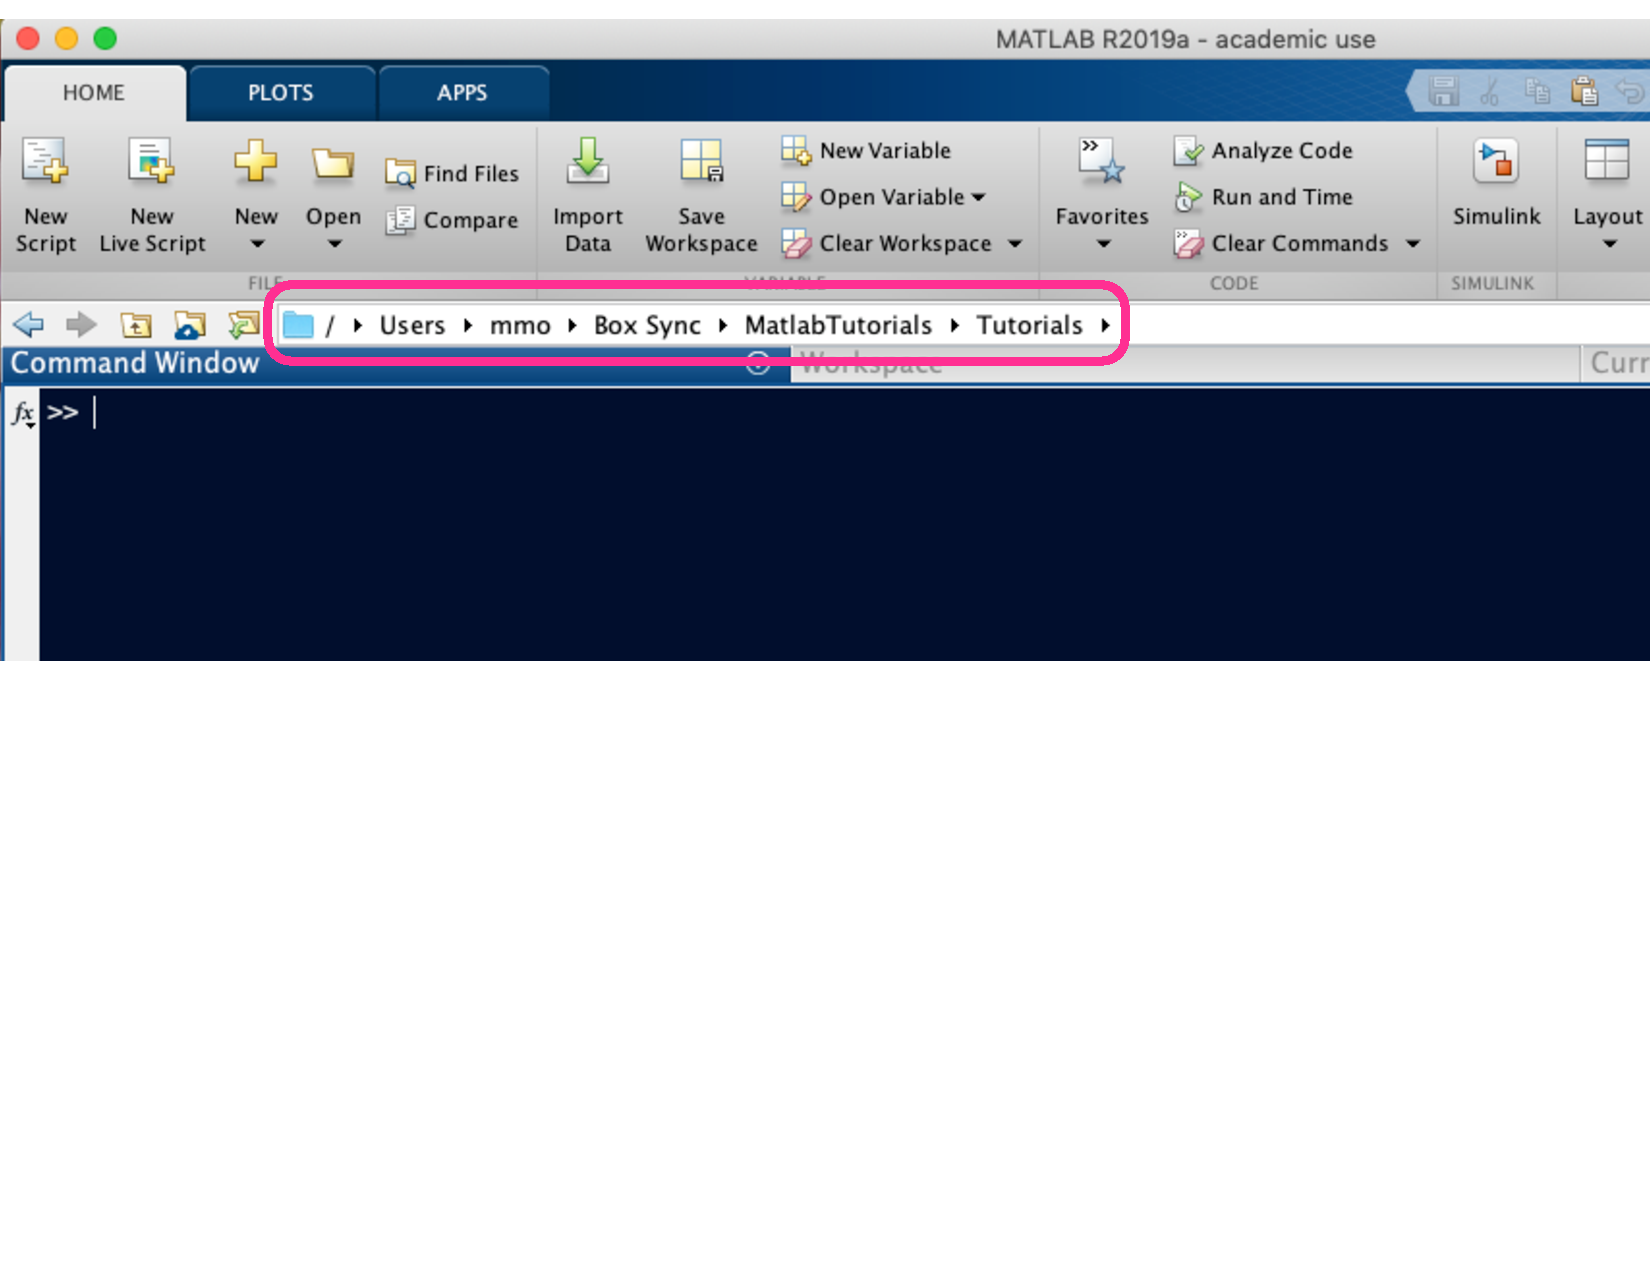
\includegraphics[width=0.8\textwidth]{Navigate_Bar.pdf}
\caption{
Navigate to the Tutorials directory using the navigation bar.
}
\end{figure}


\vspace{2mm}
\noindent
Now you can now open a Tutorial using the Open button:
\begin{figure}[h!]
\centering
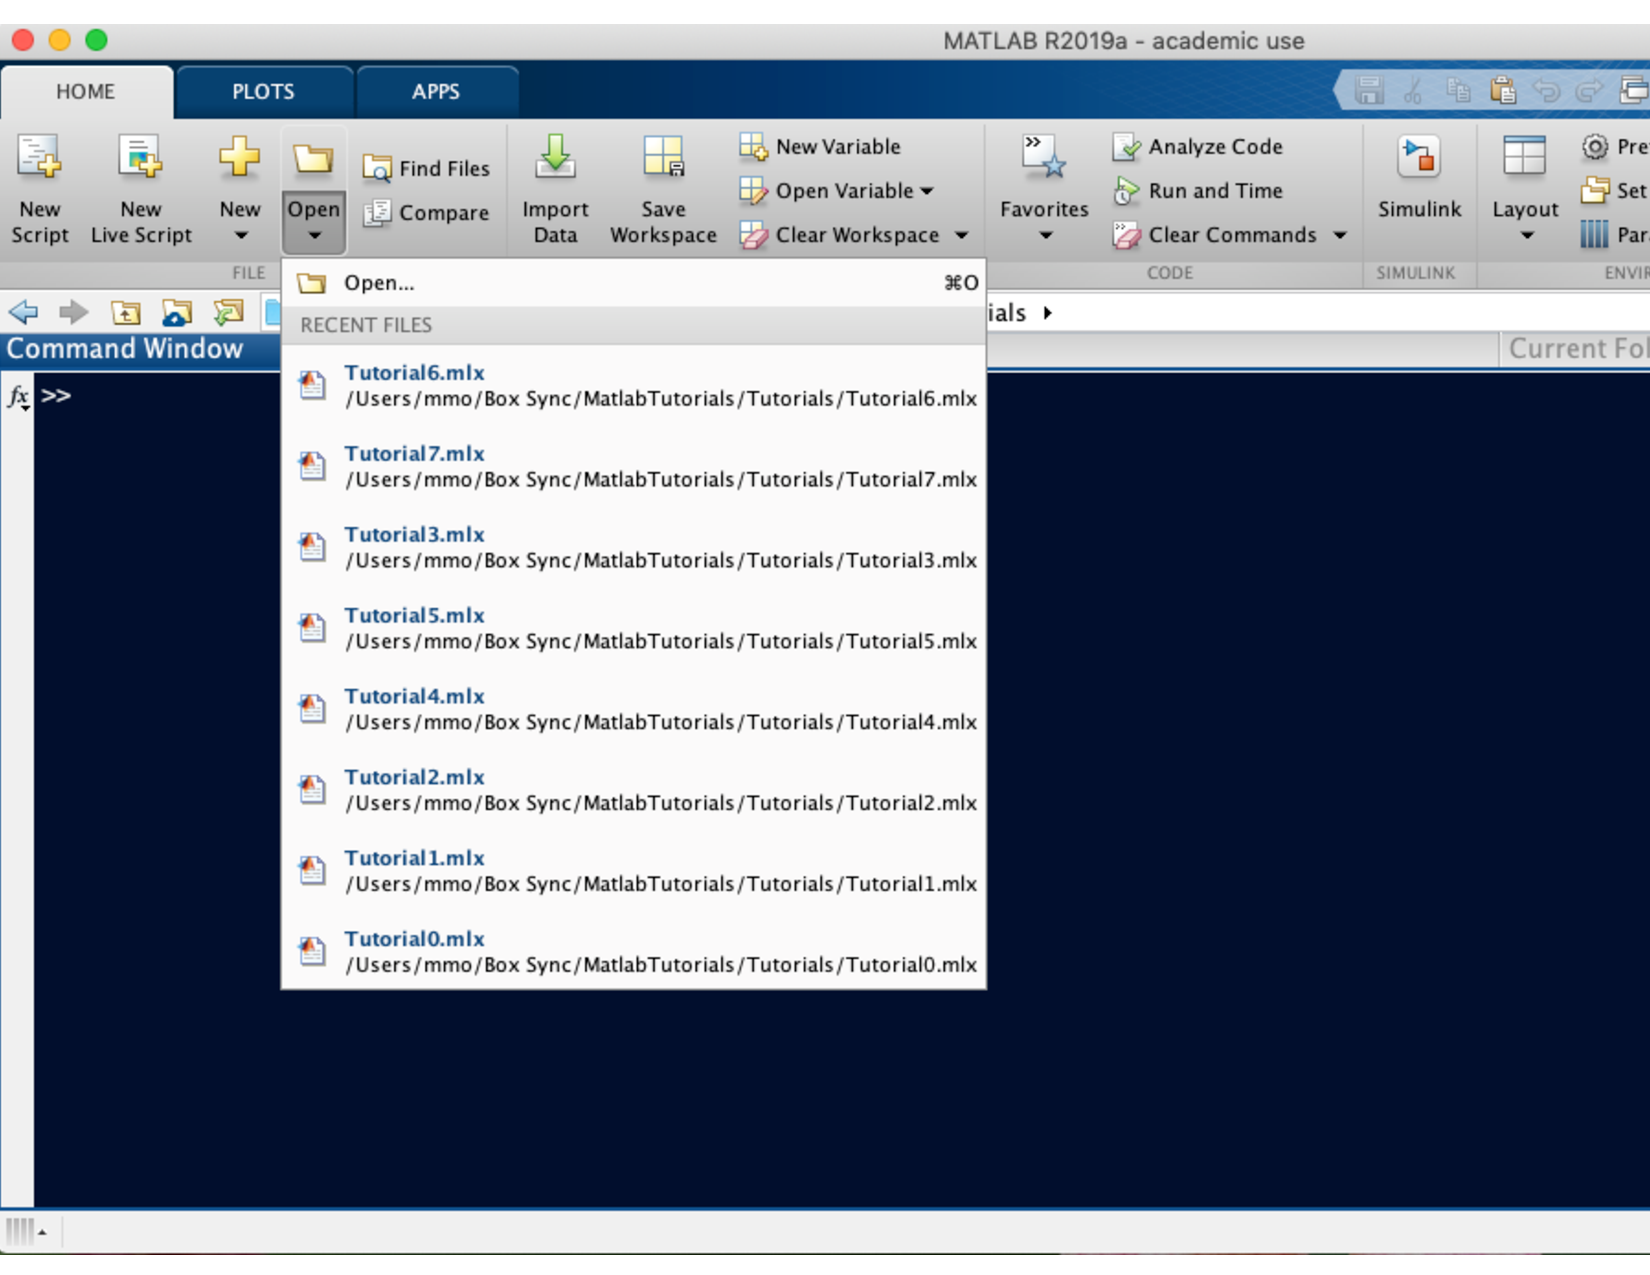
\includegraphics[width=0.8\textwidth]{Open.pdf}
\caption{
How to open a tutorial.
}
\end{figure}

\vspace{2mm}
\noindent
When you have a tutorial live-script open, it should look something like this:
\begin{figure}[h!]
\centering
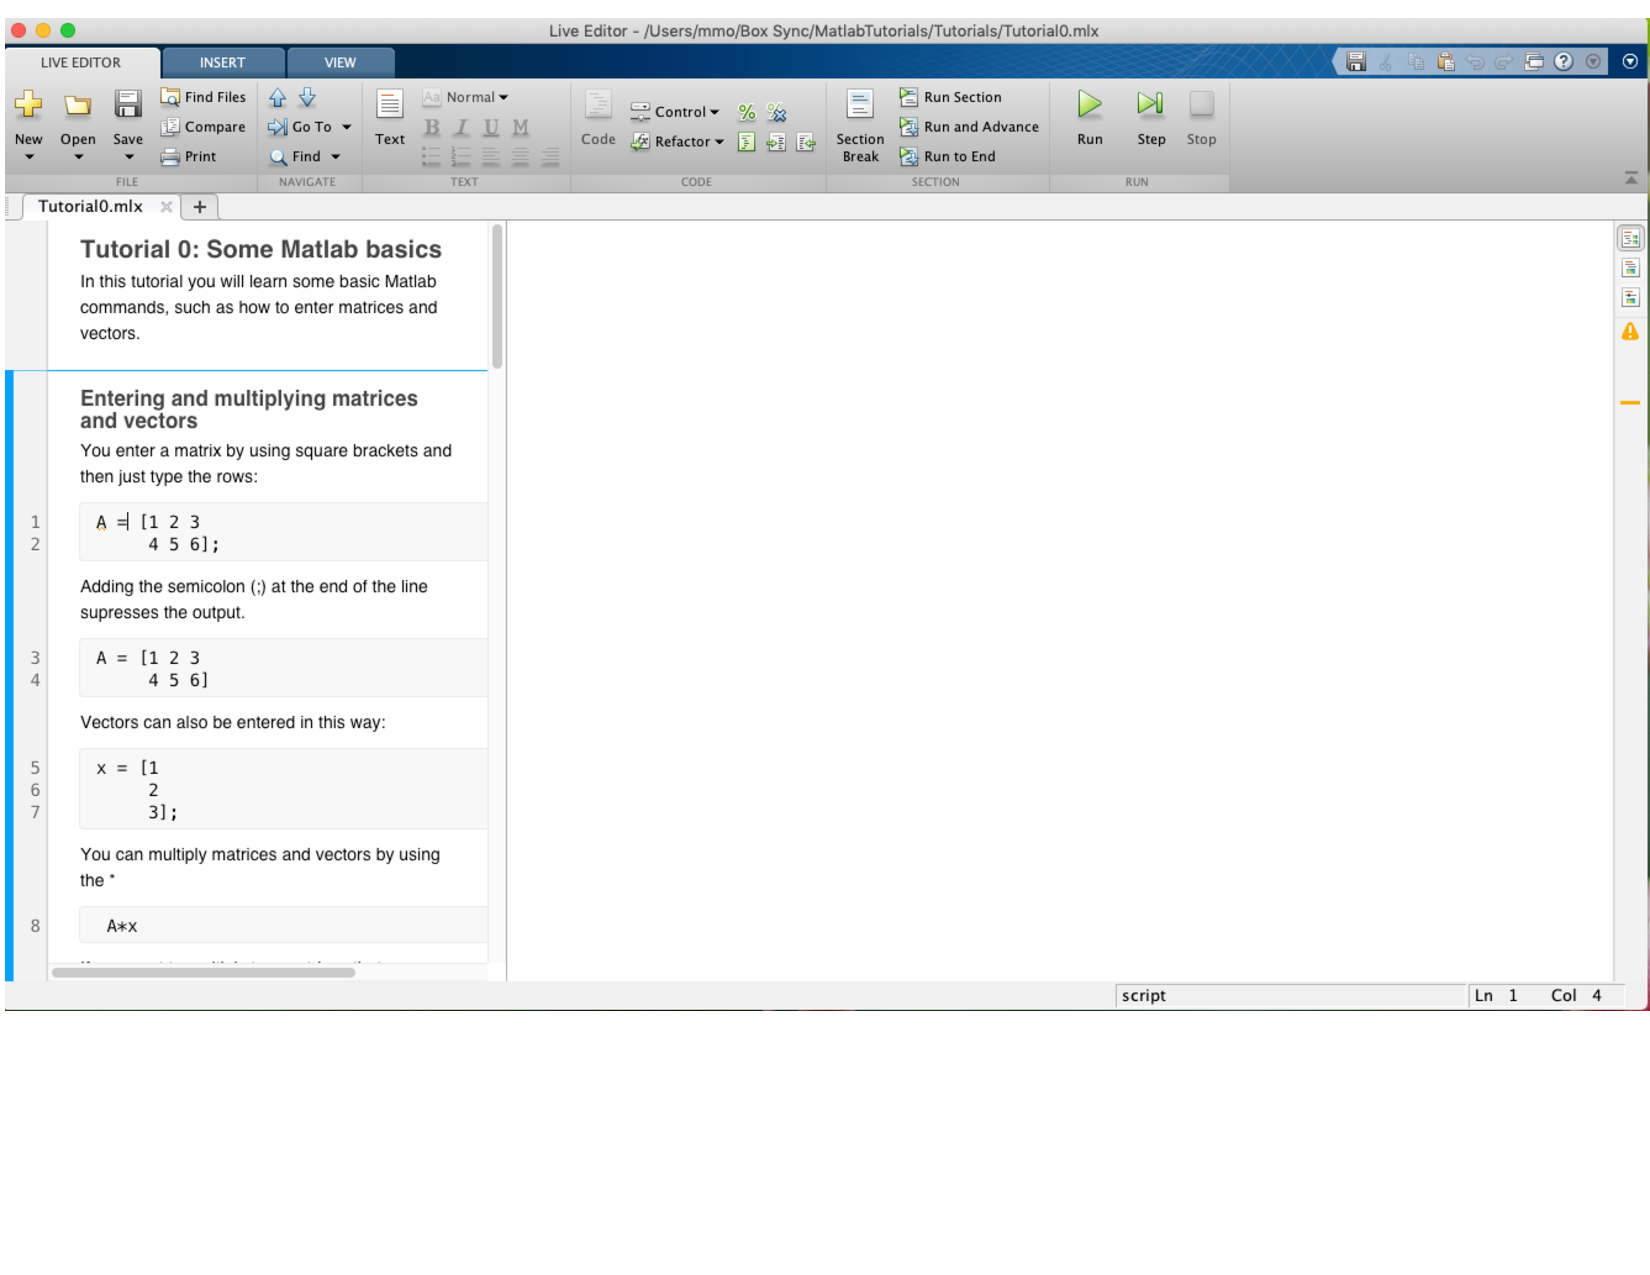
\includegraphics[width=0.8\textwidth]{OpenTutorial.pdf}
\caption{
Example of a tutorial live script.
}
\end{figure}

\newpage
\noindent
Each Tutorial is divided in a number of sections.
You can the code in one section by clicking on the light blue bar
to the left of the section. 
\begin{figure}[h!]
\centering
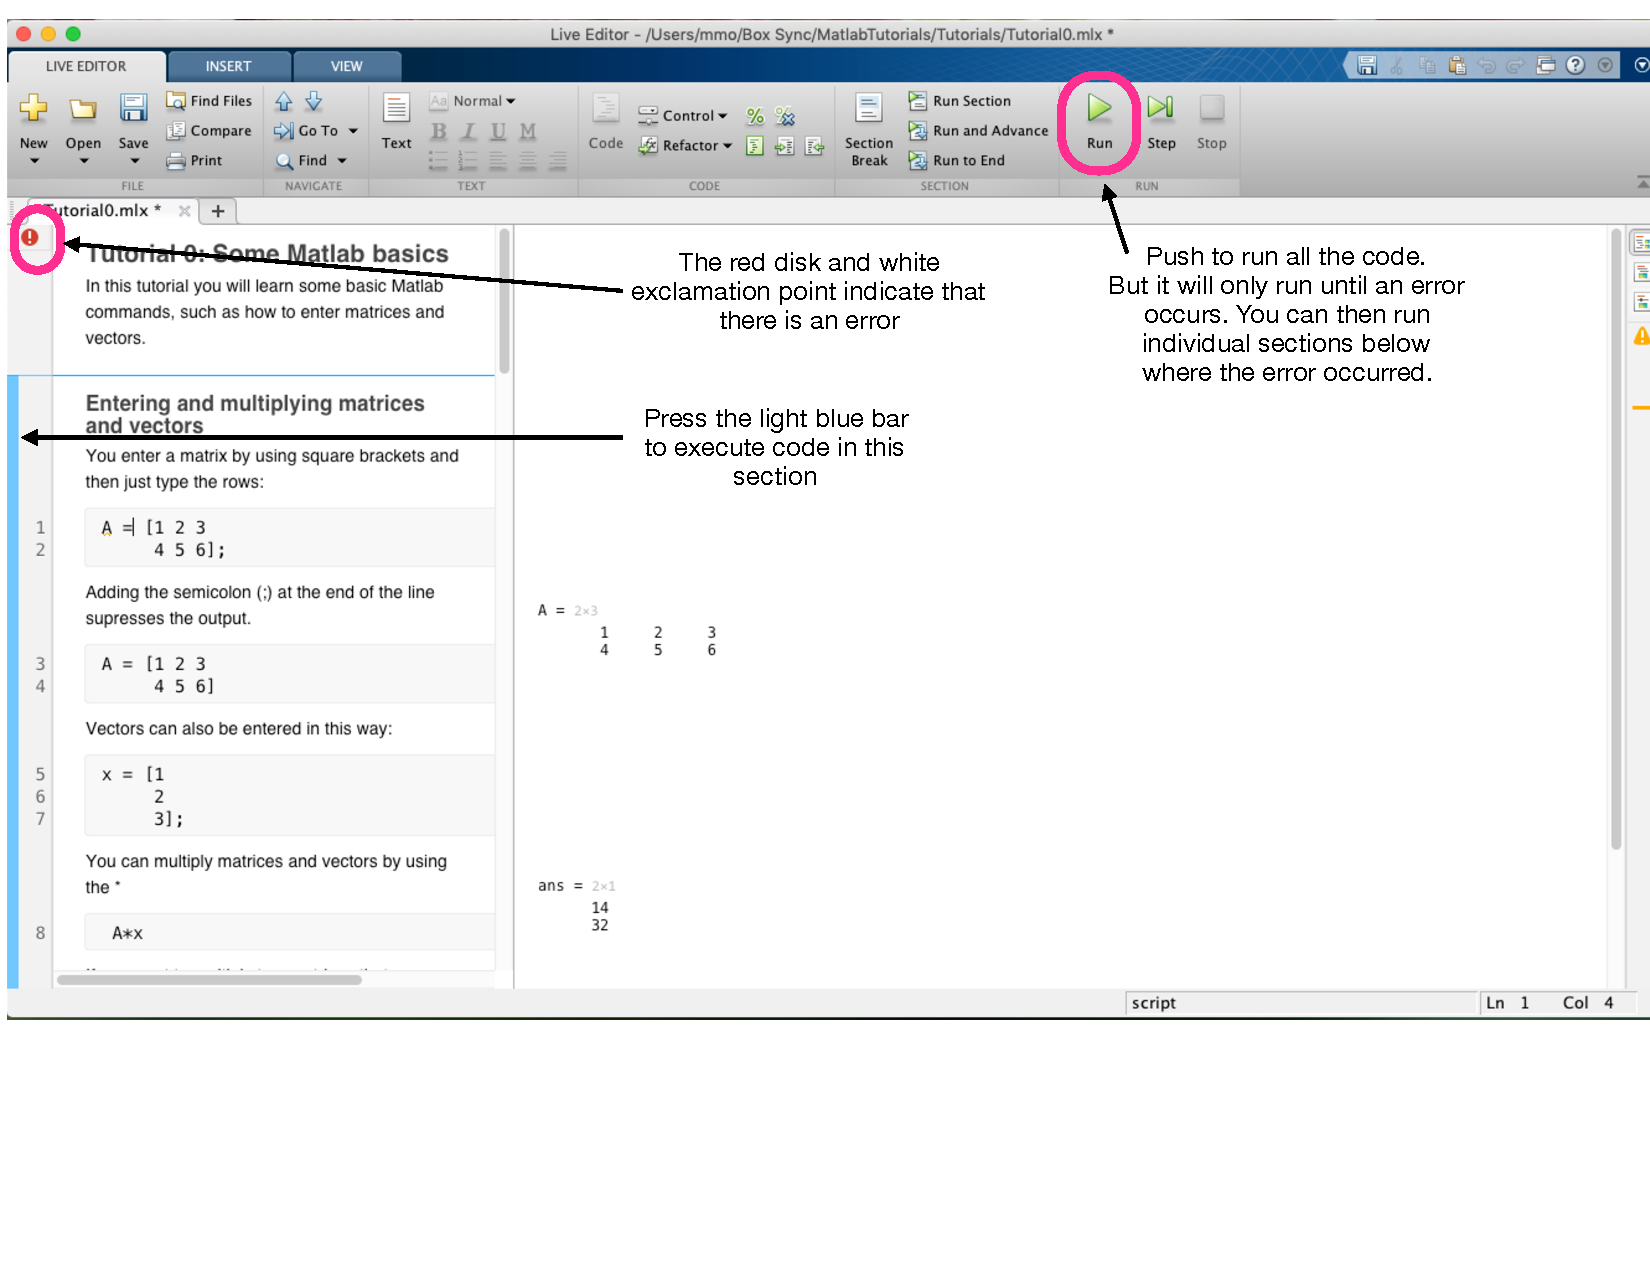
\includegraphics[width=0.8\textwidth]{RunCode.pdf}
\caption{
How to run code.
}
\end{figure}
You can also run the code in all section using the green play button
in the upper right corner of the Live-Editor bar.
Whenever an error occurs, 
a red disk with a white exclamation mark will appear in the upper left corner.
In some Tutorials, error occur on purpose (to show, for example,
that you can't multiply any two matrices).
You can run the code below where the error occurred
by clicking on the light blue bar next to the code.


\vspace{2mm}
\noindent
Sometimes, it is useful or necessary to clear old outputs and computations.
You can do that by clicking on ``VIEW'', followed by clicking on
``Clear all Ouptut''. 
\begin{figure}[h!]
\centering
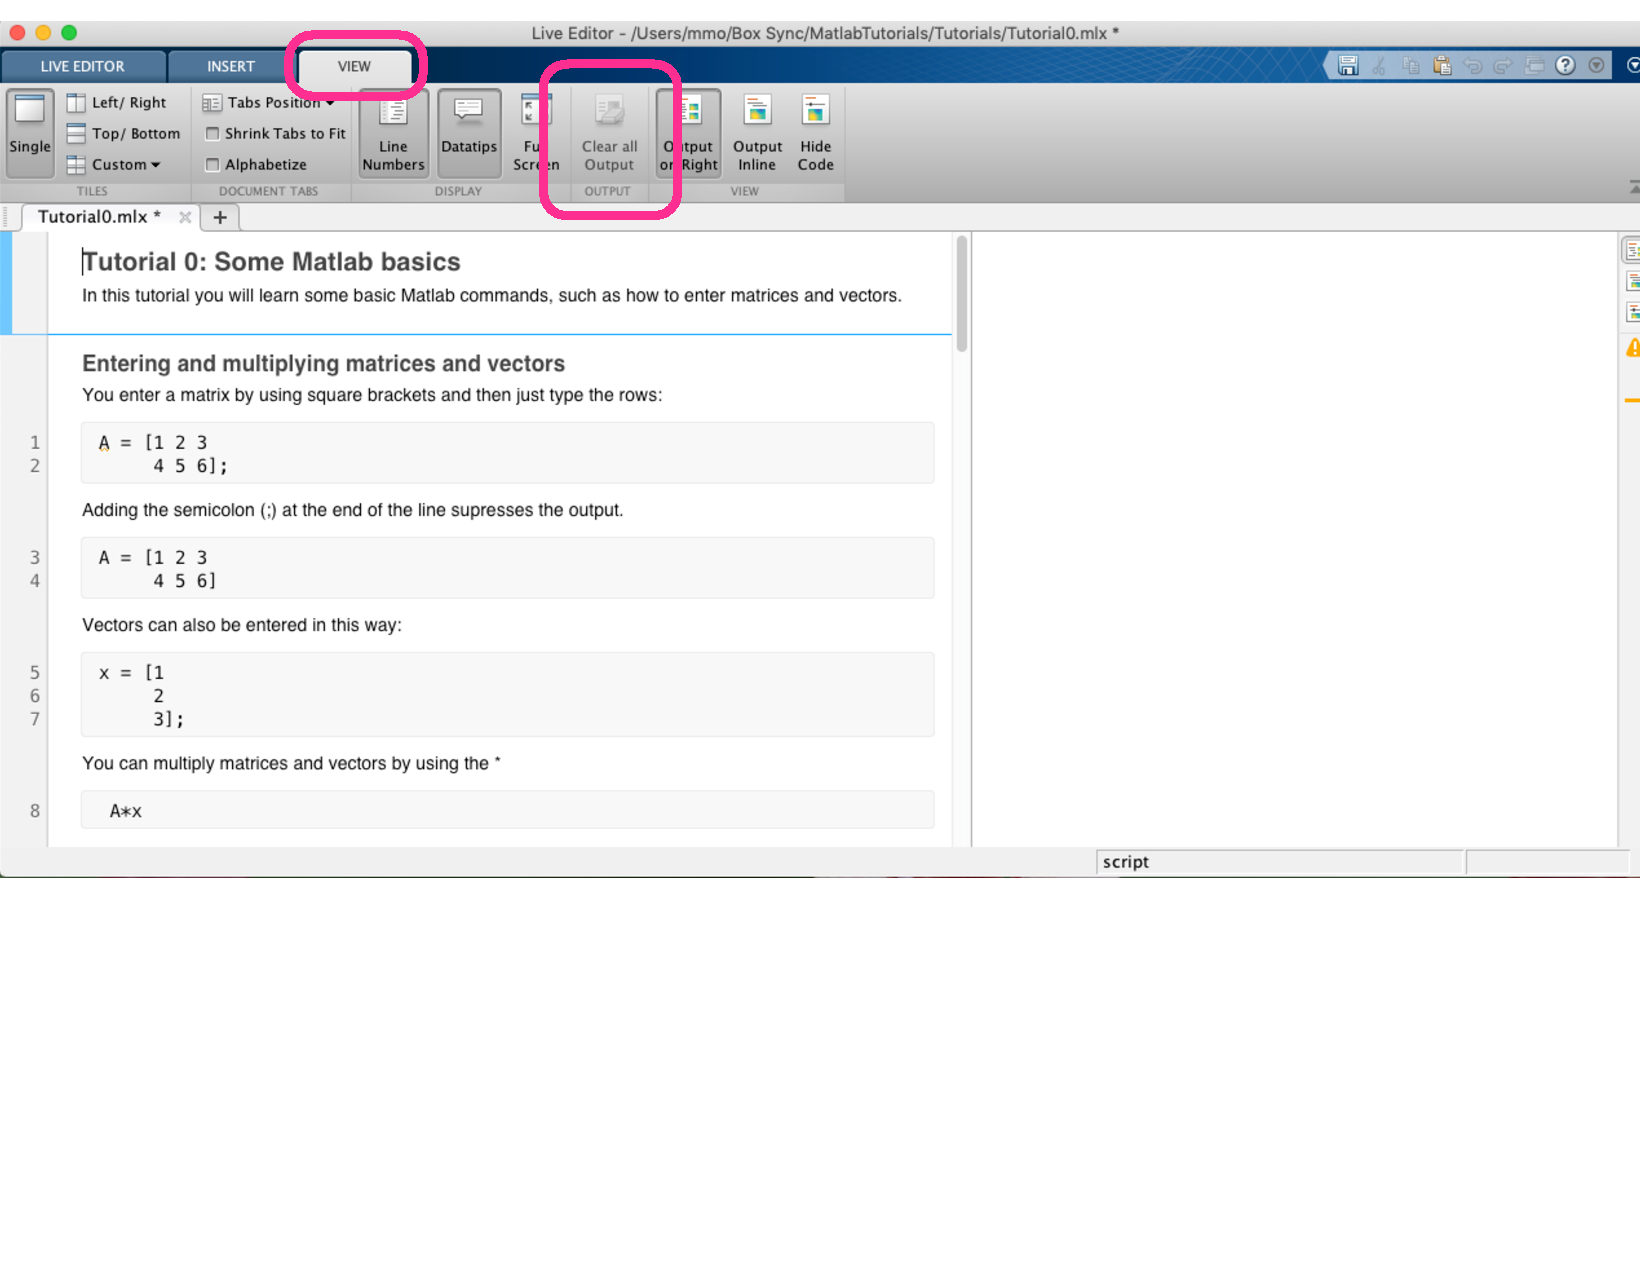
\includegraphics[width=0.8\textwidth]{Clear.pdf}
\caption{
How to clear output.
}
\end{figure}

\vspace{2mm}
\noindent
If your instructor posts solutions, 
then you can use the solutions in the same way as the tutorials.
Make sure that the Solutions are copied into the same folder
as the Tutorials that also contains the ``Data'' subdirectory.


\section{How to solve the Exercises}
At the end of each tutorial, 
you will find a few exercises.
You can work on the exercises by directly extending the live script.
You can insert code and plain text for explanations:
\begin{figure}[h!]
\centering
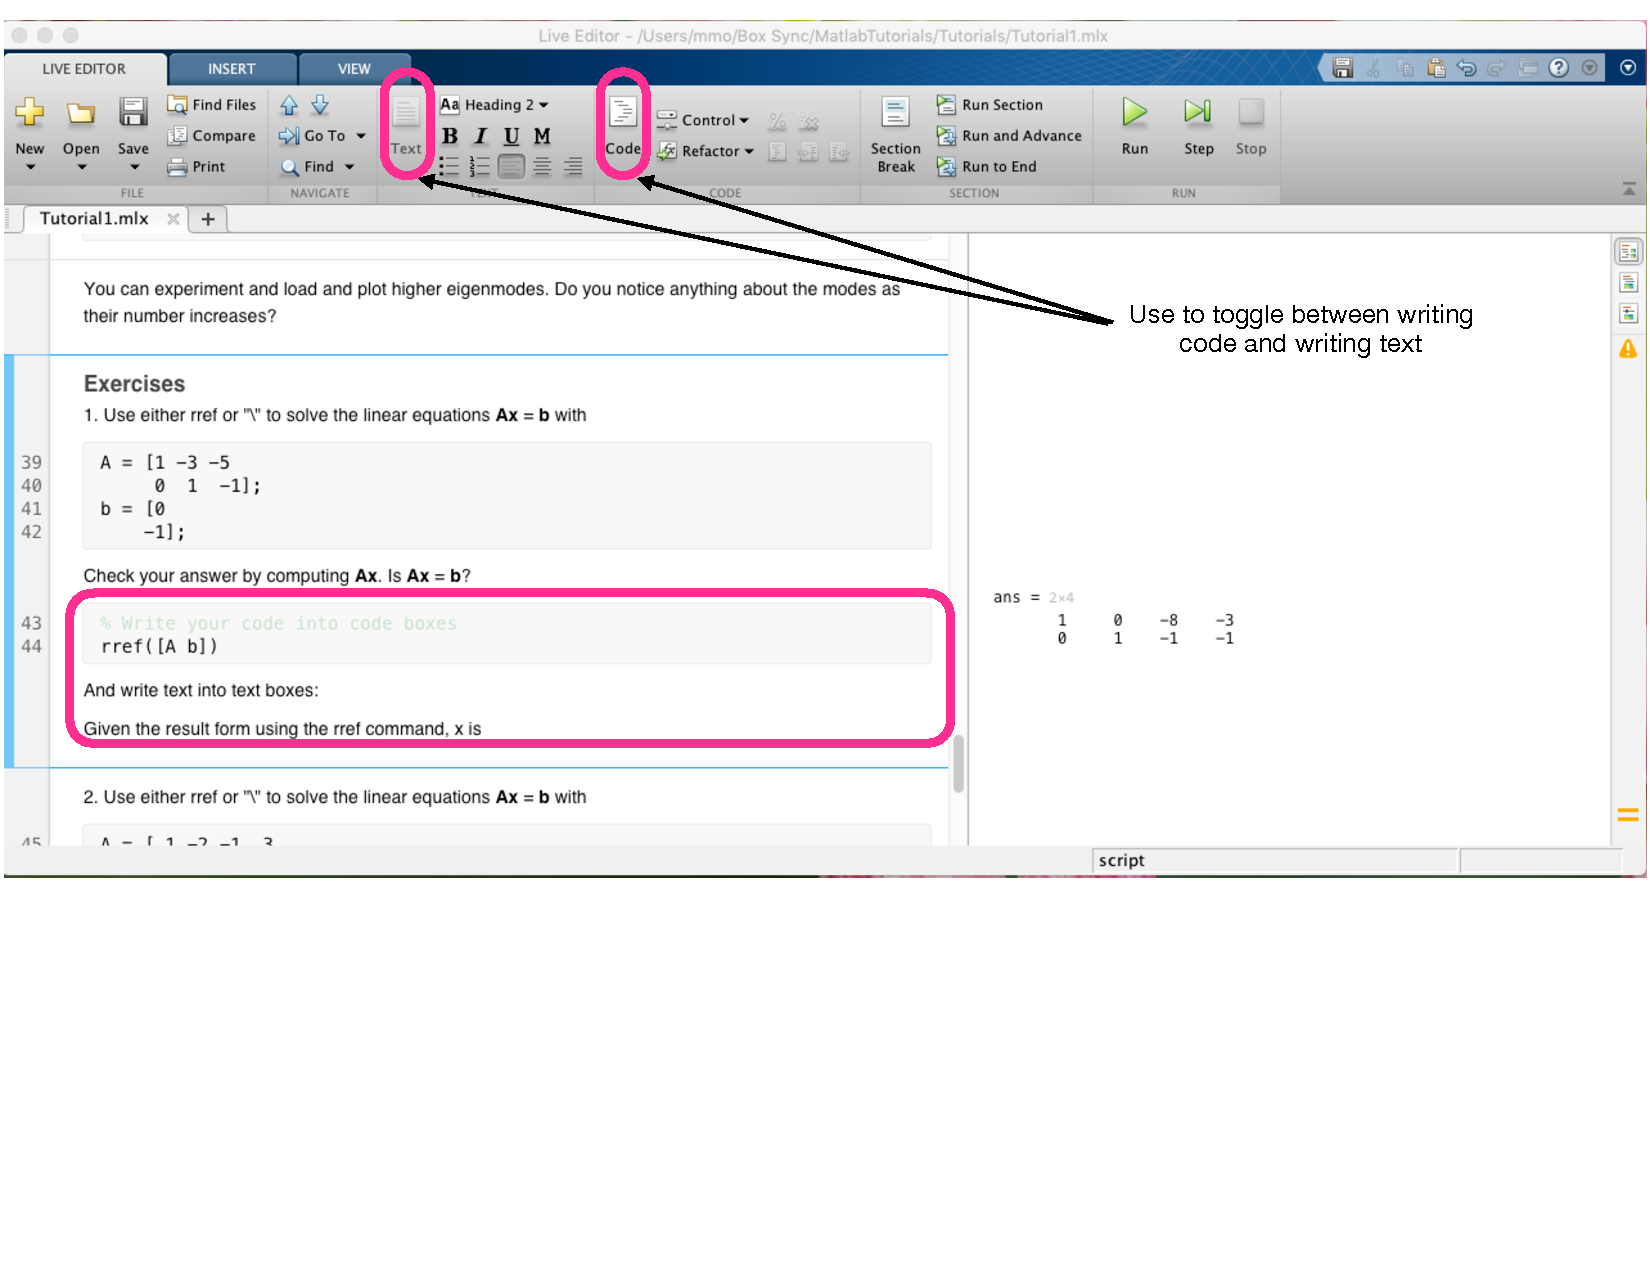
\includegraphics[width=0.8\textwidth]{Exercise.pdf}
\caption{
How to insert text and code to solve the exercises.
}
\end{figure}
You can run the code that you wrote by clicking on the light blue bar next to the section
for the exercise.

\vspace{2mm}
\noindent
Once you are done with the exercises,
you can save your work.
Find out from your instructor how the exercises are to be handed in.
There are several options. 
For example, you can make a pdf file out of your completed Tutorial using the Export function.
\begin{figure}[h!]
\centering
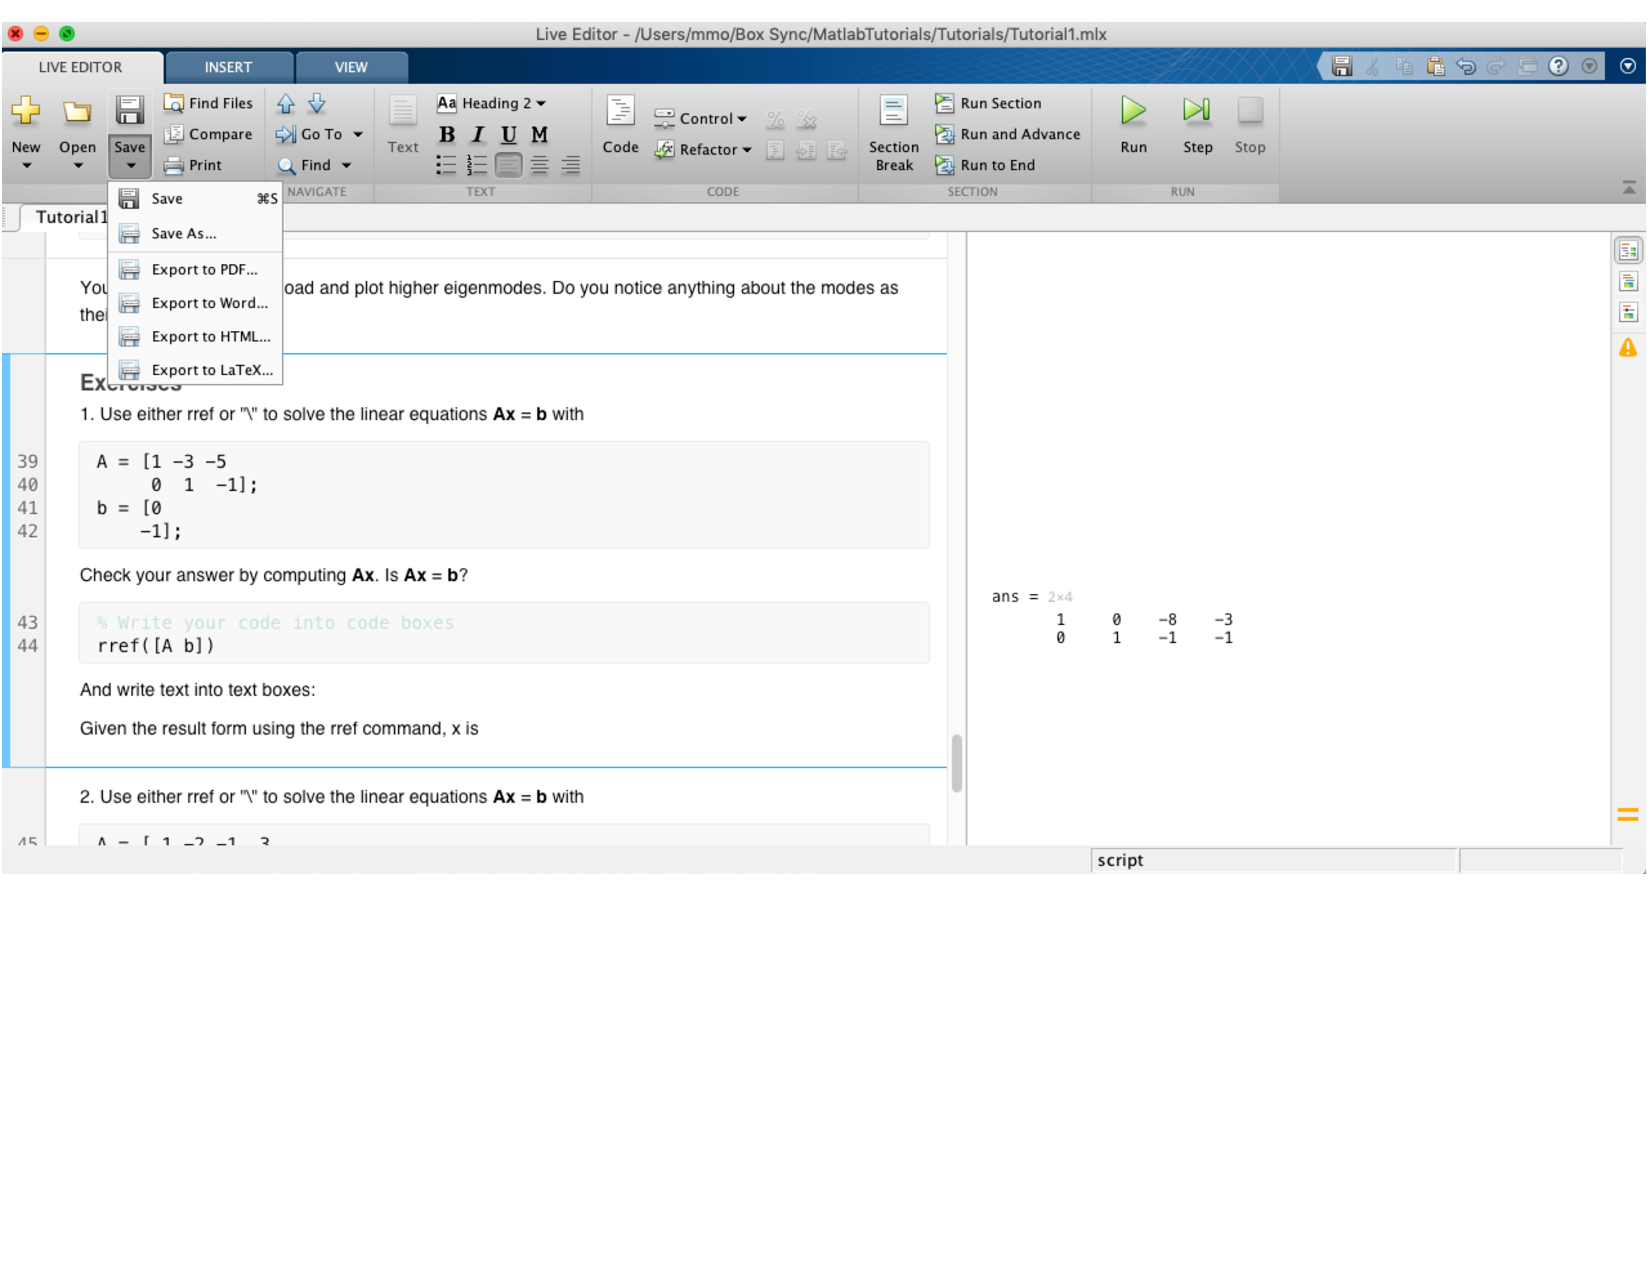
\includegraphics[width=0.8\textwidth]{Export.pdf}
\caption{
How to export your tutorial with completed exercises.
}
\end{figure}

\section{Feedback, comments and questions}
If you have difficulties with running a Tutorial please contact your instructor.
Please also send feedback and general comments to your instructor
who will be able to forward these to me.

\end{document}
